
%----------------------------------------------------------------------------------------
%	CHAP Seurat
%----------------------------------------------------------------------------------------

\chapterimage{blue-chapter-head_4-reduced.pdf} % Chapter heading image

\chapter{Seurat}\label{chap:Seurat}

\section{The Seurat language}

The Seurat language consists of statements that help with the analysis of
single cell RNA-sequencing data (scRNA-seq data). These statements cover a wide range of
functionality: loading scRNA-seq data, cleaning up the data, adjusting it (by normalization
or scaling), plotting it, computing extra information based on the data (principal components, markers,
etc.), aligning data from multiple samples, performing limma analysis on it and other
functionality.

Seurat statements can be typed in an Analysis script (see Chapter~\ref{chap:Analyses}).
The simplest way to see what Seurat statements are valid at a given line in an
analysis file, is to look at the suggestions offered by the context assistant. Figure~\ref{fig:ContextAssistantBeg}
and Figure~\ref{fig:ContextAssistantMid} show two examples of context assistants.
To activate the context assistant, just press
\keys{\return} in the script to generate an empty line. Placing the cursor on the empty line should
bring up the context assistant; in case you do not see it, press \keys{\space} on the empty line.
Moreover, to see all possible statements, you can use auto-completion like for all other
statements in a script (see Chapter~\ref{chap:Analyses}).

\begin{SCfigure}
  \centering
  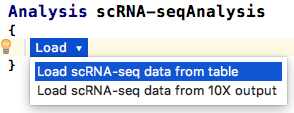
\includegraphics[width=\figWidthTiny]{figures/ContextAssistantBeg.png}
    \caption[Context assistant at beginning of script.]{\textbf{Context assistant at
    beginning of script.} At the beginning of the script, the
    context assistant suggests loading a Seurat object either directly from the output
    of the 10X, or from an expression table.}
\label{fig:ContextAssistantBeg}
\end{SCfigure}

\begin{figure}[h!tbp]
  \centering
  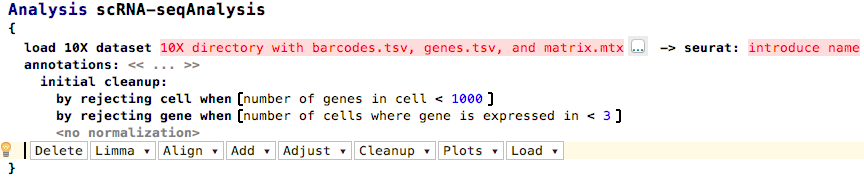
\includegraphics[width=\figWidthWide]{figures/ContextAssistantMid.png}
    \caption[Context assistant after loading one Seurat object.]{\textbf{Context
    assistant after loading one Seurat object.} Once we have Seurat objects
    available in the script, more Seurat statements become valid.}
\label{fig:ContextAssistantMid}
\end{figure}

To start writing analyses using Seurat, you need to import devkit
\texttt{org\allowbreak.campagne\allowbreak{}lab\allowbreak.metaR}
and language \texttt{org\allowbreak.campagne\allowbreak{}lab\allowbreak.metar\allowbreak.seurat}.
\noindent The following sections describe the kinds of statements offered by the MetaR
\texttt{org\allowbreak.campagne\allowbreak{}lab\allowbreak.metar\allowbreak.seurat} language.
In these sections, we talk about Seurat objects, but you have to keep in mind that a Seurat
object is a structure that stores scRNA-seq data.

\section{Loading Seurat objects}
There are two statements in the Seurat language for loading a Seurat object, one directly
from the files produced by 10X, and one from an expression matrix.

\subsection{Load 10X dataset}\label{subsec:Load10XDataset}
The \texttt{load 10X dataset} statement makes it possible to load a Seurat object directly
from the output files of 10X Genomics. The Seurat object and its properties become available
to the statements that follow the loading (until the line where it is deleted; see
Section~\ref{sec:OtherSeuratStatements}). You can create this statement by clicking
\menu{Load > Load scRNA-seq data from 10X output} in the context assistant, or by typing
the alias \texttt{load 10X dataset} on an empty line of Analysis (see Figure~\ref{fig:Load10XDataset})
for a new load 10X dataset statement).

\begin{figure}[h!tbp]
  \centering
  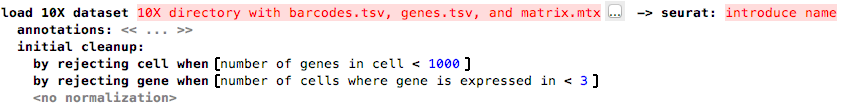
\includegraphics[width=\figWidthWide]{figures/Load10XDataset.png}
    \caption[New load 10X dataset statement.]{\textbf{New load 10X dataset statement.}
    Use this statement to load a Seurat object from the output of 10X Genomics.}
\label{fig:Load10XDataset}
\end{figure}

When creating a new \texttt{load 10X dataset} statement, the \texttt{by rejecting cell when}
strategy and \texttt{by rejecting gene when} come prefilled by default with certain upper
thresholds, but these strategies can be changed.

\paragraph{input directory} This field of \texttt{load 10X dataset} should point to
the directory produced by 10X Genomics that contains the following three files: ``barcodes.tsv",
``genes.tsv" and ``matrix.mtx". Unless the directory you specify exists on the disk and it contains
these three files, the input directory field will be shown on a red background. Notice that
this field has a button to let you select the directory.

\paragraph{annotations} The annotations are references to group usages (see
Section~\ref{sec:ColumnGroupUsage}). They allow you to attach more information to
the data loaded from 10X Genomics. For instance, if you load data that corresponds
to a certain patient and a certain state of the sample (condition),
you would annotate the Seurat object with a reference to a group usage that represents the
patient and with a reference to a group usage that represents the state (see
Figure~\ref{fig:ExampleLoad10XDataset}).
These annotations are used by the expression tables generated from the Seurat object
in the limma statements (see Section~\ref{sec:LimmaSeurat}). Note that you
need to create groups and group usages in a Column Group Container root node
in the model of your solution. If a Column Group Container does not exist in
the model, than you have to create one (see Section~\ref{sec:ColumnGroupContainer}).

\paragraph{cleanup strategies}
There are three possible strategies available when loading data from 10X Genomics: rejecting
a cell whose number of genes is lower or higher than a threshold, rejecting a
gene when the number of cells it appears in is greater or smaller than a threshold, and
normalizing the data at loading time. The cleanup strategies are explained in
Section~\ref{sec:CleanupSeurat}.

\paragraph{output} The output of the \texttt{load 10X dataset} statement is a Seurat object.
You need to set the name of this object.

\paragraph{Example} Figure~\ref{fig:ExampleLoad10XDataset} presents an example of a
\texttt{load 10X dataset} statement.

\begin{figure}[h!tbp]
  \centering
  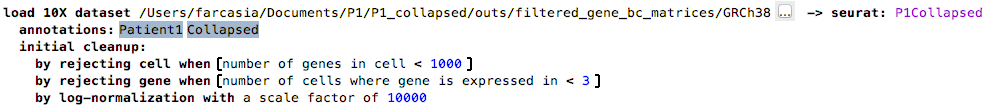
\includegraphics[width=\figWidthWide]{figures/ExampleLoad10XDataset.png}
    \caption[Example of load 10X dataset statement.]{\textbf{Example of load 10X dataset statement.}
    In this example, we load data for a patient denoted ``Patient1", from a sample of collapsed
    tubules tissue. As a result, we annotate this Seurat object with ``Patient1" and
    ``Collapsed". Furthermore, we reject the cells with less than 1000 genes expressed in
    them, and the genes that can only be found in less than 3 cells. Finally, we normalize
    the data using a scale factor of 10000.}
\label{fig:ExampleLoad10XDataset}
\end{figure}

\subsection{Load dataset from table}
The \texttt{load dataset from} statement makes it possible to load a Seurat object from a
table that contains expression data. You can create this statement by clicking
\menu{Load > Load scRNA-seq data from table} in the context assistant, or by typing
the alias \texttt{load dataset from table} on an empty line of Analysis. This statement
is identical in fields and behavior to the \texttt{load 10X dataset} statement, except
for the place of input (one is a directory generated by 10X Genomics, and one is a table).
Thus, we refer you to Subsection~\ref{subsec:Load10XDataset} for further details on the common fields.

\paragraph{input table}
The input table should have genes on the rows and cells on the columns.
Moreover, the table should have the row names. To reference a table
from this statement, you need to have a table available in the model (either by importing
it, or by obtaining it from other statements; see Section~\ref{chap:Tables}).

\paragraph{Example} Figure~\ref{fig:ExampleLoadTable} presents an example of a
\texttt{load data from table} statement.

\begin{figure}[h!tbp]
  \centering
  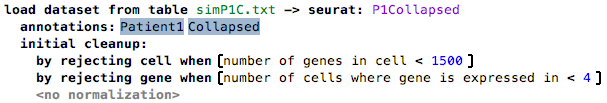
\includegraphics[width=\figWidthWide]{figures/ExampleLoadTable.png}
    \caption[Example of load data from table statement.]{\textbf{Example of load data from table statement.}
    In this example, we load data from a table with simulated data for a pacient
    denoted ``Patient1", and from a sample of collapsed tubules tissue.
    As a result, we annotate the Seurat object with ``Patient1" and
    ``Collapsed". Furthermore, we reject the cells with less than 1500 genes expressed in
    them, and the genes that can only be found in less than 4 cells. We do not normalize
    the data at loading time.} 
\label{fig:ExampleLoadTable}
\end{figure}


\section{Cleaning up Seurat objects}\label{sec:CleanupSeurat}
\subsection{Reject gene strategy}
\subsection{Reject cell strategy}
\subsection{Regress out strategy}
\subsection{Accept highly variable genes strategy}
\subsection{Normalization strategy}

\section{Adjusting Seurat objects}
\subsection{Normalize Seurat object}
\subsection{Scale Seurat object}

\section{Plotting Seurat objects}
\subsection{Diagnostic plots}
\subsection{Features plot}
\subsection{Features and total plot}

\section{Adding information to Seurat objects}
\subsection{Add principal component information}
\subsection{Add clusters information}
\subsection{Add markers information}

\section{Aligning Seurat objects}
\subsection{Pre-align Seurat objects}
\subsection{Align Seurat object}

\section{Limma for Seurat objects}\label{sec:LimmaSeurat}
\subsection{Pre-limma Seurat object}
\subsection{Limma voom}

\section{Other Seurat statements}\label{sec:OtherSeuratStatements}
\subsection{Merge Seurat objects}
\subsection{Delete Seurat object}
